\documentclass[a4paper,12pt]{extarticle}
\usepackage[utf8x]{inputenc}
\usepackage[T1,T2A]{fontenc}
\usepackage[russian]{babel}
\usepackage{hyperref}
\usepackage{indentfirst}
\usepackage{listings}
\usepackage{color}
\usepackage{xcolor}
\usepackage{here}
\usepackage{array}
\usepackage{multirow}
\usepackage{graphicx}
\usepackage{amsmath}

\hypersetup{
    colorlinks = false,
    linkbordercolor = {white}
}

\definecolor{string}{HTML}{B40000} % цвет строк в коде
\definecolor{comment}{HTML}{008000} % цвет комментариев в коде
\definecolor{keyword}{HTML}{1A00FF} % цвет ключевых слов в коде
\definecolor{morecomment}{HTML}{8000FF} % цвет include и других элементов в коде
\definecolor{сaptiontext}{HTML}{FFFFFF} % цвет текста заголовка в коде
\definecolor{сaptionbk}{HTML}{999999} % цвет фона заголовка в коде
\definecolor{bk}{HTML}{FFFFFF} % цвет фона в коде
\definecolor{frame}{HTML}{999999} % цвет рамки в коде
\definecolor{brackets}{HTML}{B40000} % цвет скобок в коде

\usepackage{caption}
\renewcommand{\lstlistingname}{Программа} % заголовок листингов кода

\bibliographystyle{ugost2008ls}

\usepackage{listings}
\lstset{ %
	extendedchars=\true,
	keepspaces=true,
	language=Python,						% choose the language of the code
	% Цвета
	keywordstyle=\color{keyword}\ttfamily\bfseries,
	%stringstyle=\color{string}\ttfamily,
	stringstyle=\ttfamily\color{red!50!brown},
	commentstyle=\color{comment}\ttfamily\itshape,
	morecomment=[l][\color{morecomment}]{\#},
	basicstyle=\footnotesize,		% the size of the fonts that are used for the code
	numbers=left,					% where to put the line-numbers
	numberstyle=\footnotesize,		% the size of the fonts that are used for the line-numbers
	stepnumber=1,					% the step between two line-numbers. If it is 1 each line will be numbered
	numbersep=5pt,					% how far the line-numbers are from the code
	backgroundcolor=\color{white},	% choose the background color. You must add \usepackage{color}
	showspaces=false				% show spaces adding particular underscores
	keywordstyle=color{blue}\bfseries, 
	showstringspaces=false,			% underline spaces within strings
	showtabs=false,					% show tabs within strings adding particular underscores
	frame=single,          		% adds a frame around the code
	tabsize=2,						% sets default tabsize to 2 spaces
	captionpos=t,					% sets the caption-position to top
	breaklines=true,				% sets automatic line breaking
	breakatwhitespace=false,		% sets if automatic breaks should only happen at whitespace
	escapeinside={\%*}{*)},			% if you want to add a comment within your code
	postbreak=\raisebox{0ex}[0ex][0ex]{\ensuremath{\color{red}\hookrightarrow\space}},
	texcl=true,
	inputpath=listings,                     % директория с листингами
}

\usepackage[left=2cm,right=2cm,
top=2cm,bottom=2cm,bindingoffset=0cm]{geometry}

%% Нумерация картинок по секциям
\usepackage{chngcntr}
\counterwithin{figure}{section}
\counterwithin{table}{section}

%%Точки нумерации заголовков
\usepackage{titlesec}
\titlelabel{\thetitle.\quad}
\usepackage[dotinlabels]{titletoc}

%% Оформления подписи рисунка
\addto\captionsrussian{\renewcommand{\figurename}{Рисунок}}
\captionsetup[figure]{labelsep = period}

%% Подпись таблицы
\DeclareCaptionFormat{hfillstart}{\hfill#1#2#3\par}
\captionsetup[table]{format=hfillstart,labelsep=newline,justification=centering,skip=-10pt,textfont=bf}

%% Путь к каталогу с рисунками
\graphicspath{{fig/}}

\begin{document}	% начало документа

% Титульная страница
%\begin{titlepage}	% начало титульной страницы

	\begin{center}		% выравнивание по центру

		Санкт-Петербургский Национально Исследовательский Университет\\
		информационных технологий, механики и оптики \\
		Кафедра систем управления и информатики\\[3cm]
		% название института, затем отступ 6см
		
		\huge \textbf{РЕФЕРАТ}\\[0.5cm]
		\large Электромеханические системы\\[0.1cm]
		\large Система автоматического управления квадракоптера Parrot ARDrone 2.0\\[2cm]

	\end{center}


	\begin{flushright} % выравнивание по правому краю
%		\begin{minipage}{0.5\textwidth} % врезка в половину ширины текста
%			\begin{flushleft} % выровнять её содержимое по левому краю

				\large Выполнили студенты группы P3335\\
				\large А.М. Зенкин\\[0.5cm]
				\large К.В. Карпов\\[0.5cm]
				
				\large Принял  к.т.н., доцент кафедры СУиР\\
				\sign[4cm]\large  М.С. Чежин\\
				\large Оценка: \sign\\
				«\underline{\hspace{0.7cm}}» \underline{\hspace{2cm}} \the\year г.

%			\end{flushleft}
%		\end{minipage}
	\end{flushright}
	
	\vfill % заполнить всё доступное ниже пространство

	\begin{center}
	\large Санкт-Петербург\\
	\large \the\year % вывести дату
	\end{center} % закончить выравнивание по центру

\thispagestyle{empty} % не нумеровать страницу
%\end{titlepage} % конец титульной страницы
\newpage


% Содержание
% Содержание
\renewcommand\contentsname{\centerline{Содержание}}
\tableofcontents
\thispagestyle{fancy}
\newpage




\section{Цель работы}
Выборать двигатель для САУ.


\section{Варианты параметров}

$m=0,62\;kg;\;R=0,35\;m;\;$Плоскость перемещения: вертикальная\\

$g=g_0\cdot \sin(\omega t)$, где $g_0=30^{\circ}, \omega=7.5\; c^{-1}$

\section{Ход выполнения работы}
\subsection{Схема объекта управления:}
Схема объектра управления приведена на рисунке \ref{pic:pic_1}.
\begin{figure}[H]
	\begin{center}
		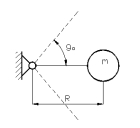
\includegraphics[scale=1.5]{3}
		\caption{- схема объекта управления} 
		\label{pic:pic_1} % название для ссылок внутри кода
	\end{center}
\end{figure}

\subsection{Расчёты требуемых параметров двигателя:}
\begin{equation}
	\begin{split}
		&J_H=mR^2=0.62\cdot 0,35^2=0.07595\; kg\cdot m^2;\\
		&\varepsilon=\dfrac{d\omega}{dt}=0.523598\cdot 7.5 = 29.4356\; red/s;\\
		&M_{Н}= mgR =2.12\; H\cdot m;\\
		&M_{TP}= M_d+M_c = 2.24+2.12= 4.36\; H\cdot m;\\
		&P_H=\left( M_H+J_H \varepsilon_M \right)\omega_M= 4.36\cdot 3.92 =17.12\;W;\\
		&P_{dv}=2P_H=17.12\cdot 2=34.24\; W;\\
	\end{split}			
\end{equation}

\newpage

\subsection{Бесколлекторный двигатель FL57BL01:}
Характеристики бесколлекторного электродвигателя приведены на рисунке \ref{pic:pic_2}.
\begin{figure}[H]
	\begin{center}
		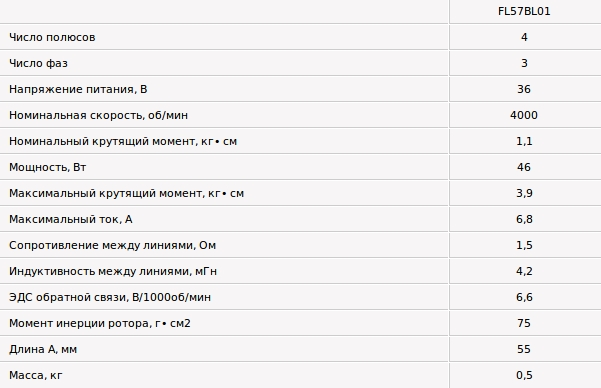
\includegraphics[scale=0.6]{2}
		\caption{- технические характеристики бесколекторного электродвигателя} 
		\label{pic:pic_2} % название для ссылок внутри кода
	\end{center}
\end{figure}

\subsubsection{Расчёт параметров двигателя:}
\begin{equation}
	\begin{split}
		&M_{eng.n}=0.1078\; Nm;\\
		&\omega_{eng.n} = 418.879\; rad/s;\\
		&J_{eng} = 0.0000075\; kg\cdot m^2;\\
		&J_p=0.2J_{eng}=0.0000015\; kg\cdot m^2;\\
	\end{split}			
\end{equation}

\subsubsection{Рассчёт оптимального передаточного числа:}
\begin{equation}
	\begin{split}
		&{M'}_H=\dfrac{M_H}{\eta}=\dfrac{0.1078}{0.8}=0.1348\; Nm;\\
		&i_0=\sqrt{\dfrac{{M'}_H+J_H \varepsilon_M}{1.2J_{eng} \varepsilon_M}} = \sqrt{\dfrac{2.79+2.2369}{1.2\cdot 0.0000075\cdot 29.45}} = 95
	\end{split}			
\end{equation}

\subsubsection{Рассчёт требуемого момента на валу двигателя:}
\begin{equation}
	\begin{split}
		&M_{req}=\left( 1.2\cdot J_{eng} +\dfrac{J_H}{i^2} \right)\cdot \varepsilon_M\cdot i + \dfrac{{M'}_H}{i};\\
		&M_{req}=\left( 1.2\cdot 7.5\cdot 10^{-6} +\dfrac{0.07595}{95^2} \right)\cdot 29.45\cdot 95 + \dfrac{0.1348}{95}=0.0501\; Nm;\\
	\end{split}			
\end{equation}

\subsubsection{Рассчёт требуемой минимальной мощности, развиваемой на валу двигателя:}
\begin{equation}
	\begin{split}
		&P_{req.min}=2\left('{M'}_H+J_H \epsilon_M\right)\omega= 2\left(0.1078+0.07595\cdot 29.45\right)\cdot 3.9269 =18.627 \; W;\\
	\end{split}			
\end{equation}

\subsubsection{Проверка перегрузочной способности и требуемой скорости:}
\begin{equation}
	\begin{split}
		&\gamma=\dfrac{M_{req}}{M_{eng.n}}=\dfrac{0.0501}{0.10787}=0.4648;\\
		&\alpha=\dfrac{i_0\omega_M}{\omega_{eng.n}}=\dfrac{95\cdot 3.9269}{418.879}=0.8906 ;\\
	\end{split}			
\end{equation}

\subsubsection{Произведём тепловой расчет по эквивалентному моменту:}
\begin{equation}
	\begin{split}
		&M_{equiv}=\sqrt{\frac{{M_{n.awg}}^2}{i}+1.2{\left( J_{eng}+\dfrac{J_{eng}}{{i}^2} \right)}^2{i_0}^2{\varepsilon_{awg}}^2}=0.5732\;H\cdot m\\
		&\varepsilon_{avg} = \dfrac{g_0\cdot \omega^2}{\sqrt{2}}=\dfrac{0.5235\cdot 7.5^2}{\sqrt{2}}=20.826\; \dfrac{rad}{c^2};\\
		&M_{equiv}=\sqrt{\frac{4.3635^2}{95}+1.2{\left( 7.5\cdot 10^{-6}+\dfrac{7.5\cdot 10^{-6}}{95^2} \right)}^2\cdot 95^2\cdot 20.826^2}=0.0575\;N\cdot m;\\
	\end{split}			
\end{equation}

\subsection{Бесколлекторный двигатель FL57BL02:}
Характеристики бесколлекторного электродвигателя приведены на рисунке \ref{pic:pic_4}.
\begin{figure}[H]
	\begin{center}
		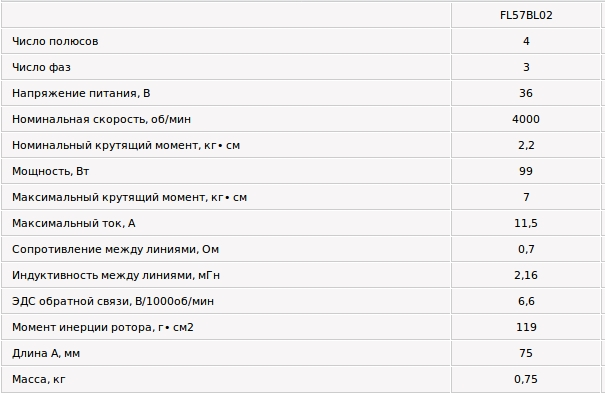
\includegraphics[scale=0.6]{4}
		\caption{- технические характеристики бесколекторного электродвигателя} 
		\label{pic:pic_4} % название для ссылок внутри кода
	\end{center}
\end{figure}

\subsubsection{Расчёт параметров двигателя:}
\begin{equation}
	\begin{split}
		&M_{eng.n}=0.2157\; Nm;\\
		&\omega_{eng.n} = 418.879\; rad/s;\\
		&J_{eng} = 0.0000119\; kg\cdot m^2;\\
		&J_p=0.2J_{eng}=0.000000238\; kg\cdot m^2;\\
	\end{split}			
\end{equation}

\subsubsection{Рассчёт требуемой мощности, развиваемой на валу двигателя:}
\begin{equation}
	\begin{split}
		&P_{req.min}=2\left({M'}_H+J_H \varepsilon_M\right)\omega=19.686 \; W;\\
	\end{split}			
\end{equation}

\subsubsection{Проверка перегрузочной способности и требуемой скорости:}
\begin{equation}
	\begin{split}
		&\gamma=\dfrac{M_{req}}{M_{eng.n}}=0.3;\\
		&\alpha=\dfrac{i_0\omega_M}{\omega_{eng.n}}=0.7218 ;\\
	\end{split}			
\end{equation}

Для выполнения поставленной задачи выбираем первый двигатель.

\subsection{Моделирование бесколлекторного электродвигателя FL57BL01:}

\subsection{Расчёт параметров математической модели и графики переходных процессов:}
\begin{equation}
	\begin{split}
		&K_Y=\frac{U_H}{U_m}=\frac{36}{10}=3.6;\\
		&K_d=\dfrac{1}{R}=\dfrac{1}{1.5}=0.667\; Om^{-1};\\
		&K_M=\dfrac{M_{eng}}{I_H}=\dfrac{0.1078}{1.277}=0.0844\; \dfrac{Nm}{A};\\
		&J_{\sum}=J_d+J_P+\dfrac{J_H}{{i_p}^2}=0.003533\;kg\cdot m^2;\\
		&K_E=\dfrac{U_H}{\omega}=\dfrac{36}{418.87}=0.0859\; \dfrac{B\cdot min}{rot};\\
		&K=\frac{K_y}{K_E\cdot i_p}=0.4409\; \dfrac{rot}{B\cdot min};\\
		&K_f=\dfrac{R}{K_MK_E{i_p}^2}=0.0229\; \dfrac{A\cdot V\cdot min\cdot Om}{N\cdot rot};\\
		&T_m=\dfrac{RJ_{\sum}}{K_MK_E} = 0.0036\; \dfrac{A\cdot V\cdot min\cdot Om\cdot kg \cdot m^2}{N\cdot rot};\\
	\end{split}			
\end{equation}

\subsection{Схема моделирования и графики переходных процессов:}
Схема моделирования бесколлекторного электродвигателя приведена на рисунке \ref{pic:pic_5}. Графики переходных процессов приведены на рисунках \ref{pic:pic_6} и \ref{pic:pic_7}.
\begin{figure}[H]
	\begin{center}
		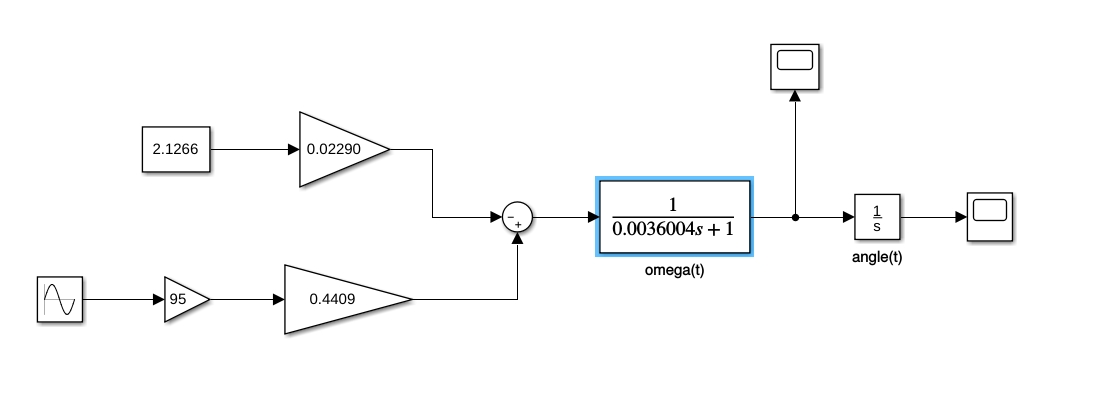
\includegraphics[scale=0.4]{5}
		\caption{- схема моделироания электромеханического двигателя} 
		\label{pic:pic_5} % название для ссылок внутри кода
	\end{center}
\end{figure}

\begin{figure}[H]
	\begin{center}
		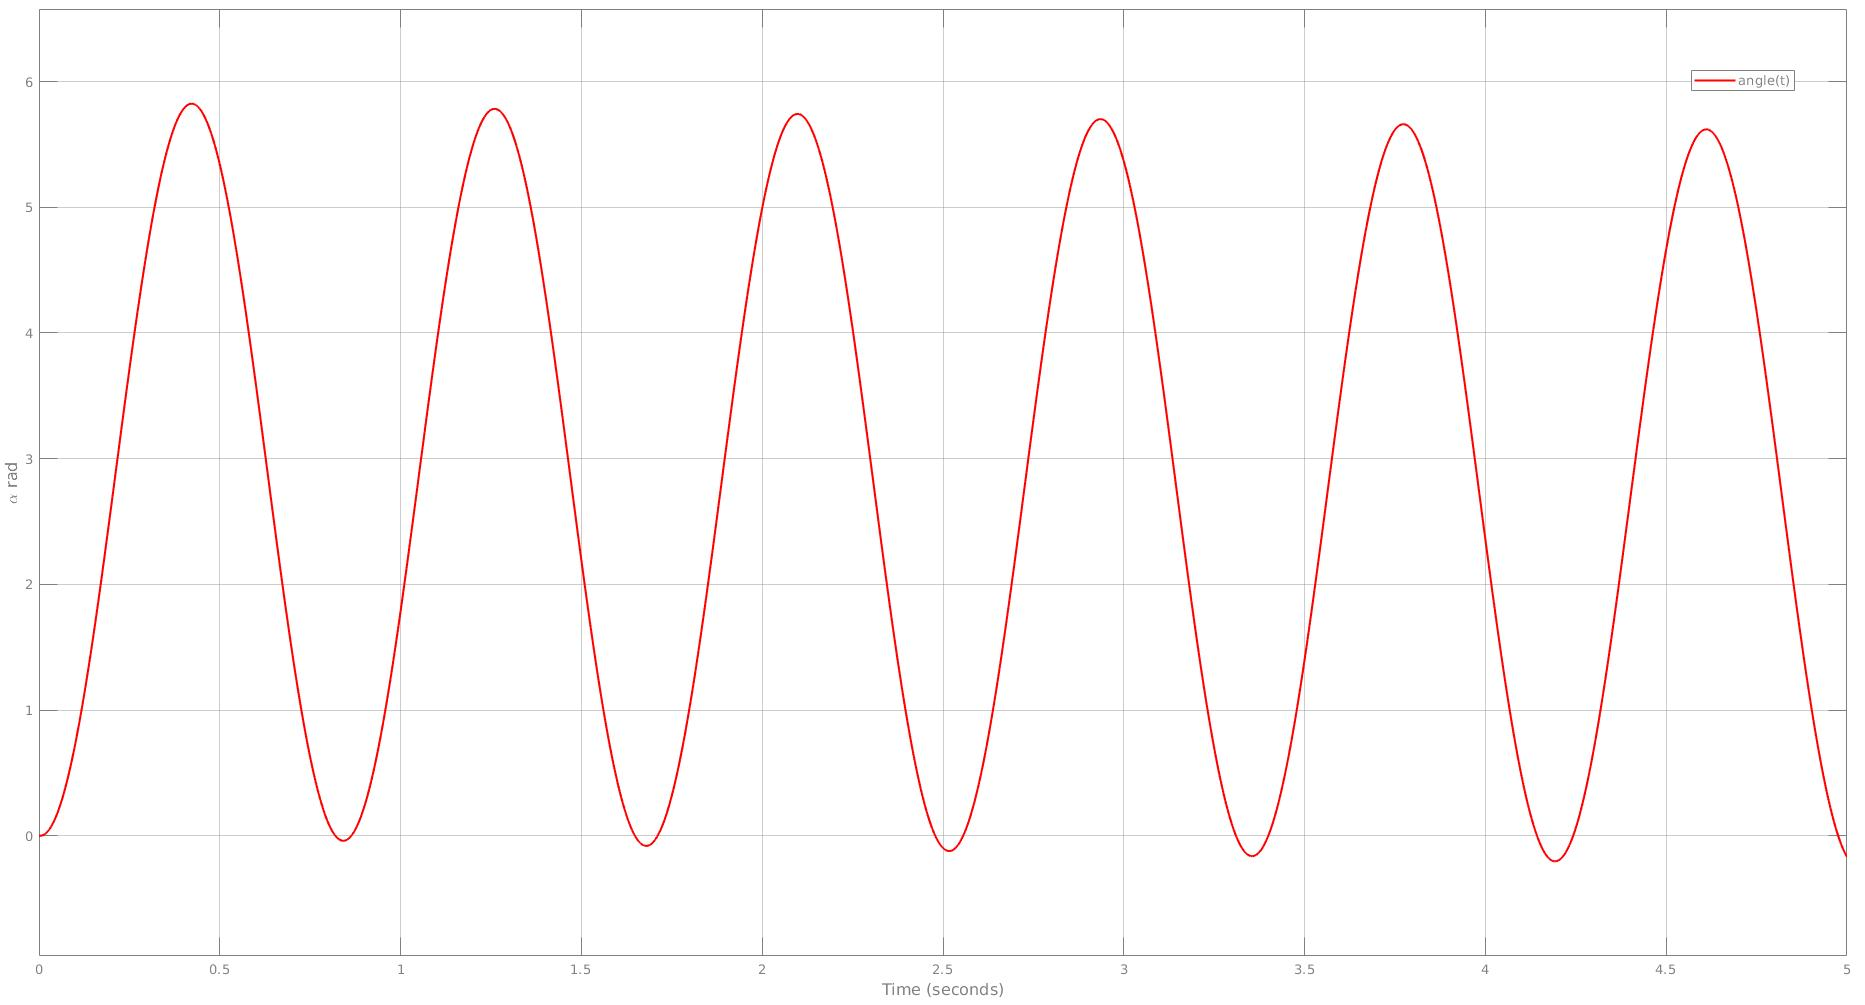
\includegraphics[scale=0.27]{sine_rot}
		\caption{- график переходного процесса alpha(t)} 
		\label{pic:pic_6} % название для ссылок внутри кода
	\end{center}
\end{figure}

\begin{figure}[H]
	\begin{center}
		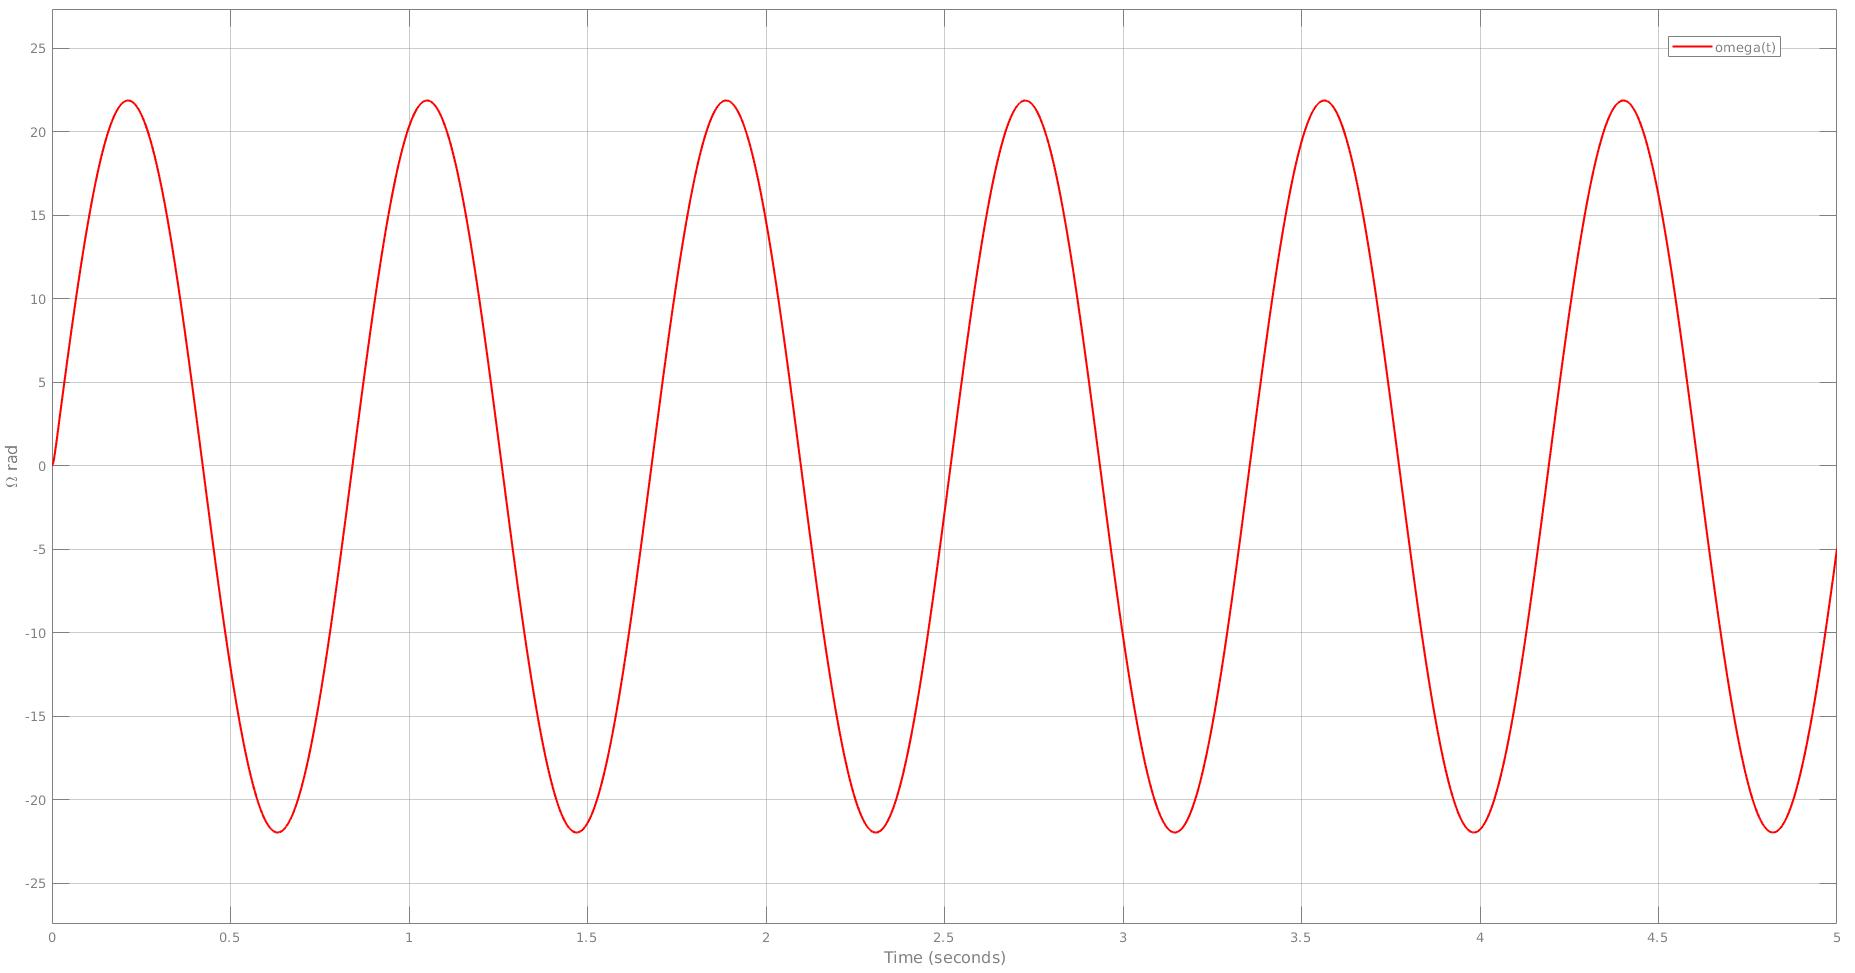
\includegraphics[scale=0.27]{12_sine_omega}
		\caption{- график переходного процесса omega(t)} 
		\label{pic:pic_7} % название для ссылок внутри кода
	\end{center}
\end{figure}

\newpage

\section{Вывод}
В данной лабораторной работе были рассмотрены два двигателя для САУ - бесколлекторного электродвигателя FL57BL01 и FL57BL02, после был выбран более подходящий двигатель для поставленной задачи - FL57BL01. Далее были построены графики переходных процессов угла и скорости от времнни. Данные графики практически полностью совпадают с условиями поставленной задачи=. Скорость отличается на 0.1 рад, а угол на 3 градуса.
\end{document}
